% $•$% !TeX root = macro_PS6_case.tex

\documentclass[]{article}
\usepackage{amssymb}
\usepackage{amsmath}
\usepackage{enumitem}
\usepackage{bm}
\usepackage{cases}
\usepackage{changepage}\usepackage{amsmath}
\usepackage{amsfonts}
\usepackage{centernot}
\usepackage{graphicx}
\usepackage{float}
\usepackage{hyperref} % to restart section numbers for different parts
\usepackage{physics} % to get partial derivatives 
\usepackage{xcolor}
\usepackage[a4paper, total={6in, 8in}]{geometry}
\usepackage{listings} % to input code
       \lstset{backgroundcolor = \color{white},
               % frame = single,
               %keywordstyle=\color{blue}
               }

%opening
\title{Econ 714 Quarter 1: Problem set 1 }
\author{Emily Case}

% command for blank footnote 
\newcommand\blfootnote[1]{%
	\begingroup
	\renewcommand\thefootnote{}\footnote{#1}%
	\addtocounter{footnote}{-1}%
	\endgroup
}

\newcount\colveccount
\newcommand*\colvec[1]{
	\global\colveccount#1
	\begin{pmatrix}
		\colvecnext
	}
	\def\colvecnext#1{
		#1
		\global\advance\colveccount-1
		\ifnum\colveccount>0
		\\
		\expandafter\colvecnext
		\else
	\end{pmatrix}
	\fi
}

\newcommand{\R}{\mathbb{R}}
\newcommand{\co}[2]{c_{#1}^{#2}} % makes subscript and superscript easier for consumption
\newcommand{\spa}{\text{ }}
\newcommand{\lnl}{\ell_n} % log likelihood function
\newcommand{\bxn}{\bar{X}_n}
\newcommand{\lag}{\mathcal{L}}
\newcommand{\sumin}{\sum\limits_{i=1}^n} % generic sumation 1 to n
\newcommand{\sumti}{\sum\limits_{t=1}^\infty} % sum - infinite horizon
\newcommand{\pin}{\Pi_{i=1}^n}
\newcommand{\argmax}{\text{arg}\max}
\newcommand{\fix} [1] {\textbf{\textcolor{blue}{#1}}} % use this to more clearly note in problem set pdf where things need to be changed. 
% end preamble

\renewcommand*{\thesection}{\arabic{section}}

\begin{document}
	
	\maketitle
	
	\blfootnote{I worked on this Problem set with Sarah Bass, Michael Nattinger, Alex von Hafften, and Danny Edgel.} 


%%%%%%%%%%%%%%%%%%%%%%%%%%%%%%%%%%%%%%%%%%%%%%%%%%%%%%%%%%
Consider a neoclassical growth model with preferences $\sum_{t=0}^\infty \beta^t U(C_t)$, production technology $F(K_t)$,  and the initial capital endowment $K_0$.  Both $U(\cdot)$ and $F(\cdot)$ are strictly increasing, strictly concave and satisfy standard Inada conditions.  The capital law of motion is \[K_{t+1}= (1-\delta)K_t+I_t-D_t\] where $D_t$ is a natural disaster shock that destroys a fixed amount of the accumulated capital.

\section{Write down the social planner’s problem and derive the intertemporal optimality condition (the Euler equation).}
Note that $F(K_t) = C_t + I_t$. Then the social planner's problem is 
\begin{align*}
\max\limits_{C_t} & \sum_{t=0}^\infty \beta^t U(C_t)  \\
\text{s.t.}\; & F(K_t)  = C_t + K_{t+1} -(1-\delta)K_t +D_t 
    % the output of a period has to cover the consumption of that period, along with the capital bought for next period, not including the disaster shock. 
\end{align*}
Now we can set up the lagrangian:
\[\sum_{t=0}^\infty \beta^t \left[ U(C_t)+ \lambda_t (-F(K_t) + C_t + K_{t+1} -(1-\delta)K_t +D_t )\right]\]
FOC with respect to $C_t$:
\[U'(C_t) + \lambda^t = 0 \]
FOC with respect to $K_{t+1}$:
\[\beta^t\lambda_t = \beta^{t+1}\lambda_{t+1} [F'(K_{t+1})+1-\delta]
\]
Simplifying and combining FOC, we can get the Euler Equation:
\[U'(C_t) = \beta U'(C_{T+1}) [F'(K_{t+1})+1-\delta]
\]

\section{Given  the  steady-state  value  of $D\ge 0$,  write  down  the  system  of  equations  that determines  the  values  of  capital $\bar{K}(D)$ and  consumption $\bar{C}(D)$  in  the  steady  state. Draw  a  phase  diagram  with  capital  in  the  horizontal  axis  and  consumption  in  the vertical  axis,  show  the  steady  states,  draw  the  arrows  representing the direction of change, and the saddle path.}
Let $K_t = K_{t+1}=\bar{K}$ and $C_t= C_{t+1}=\bar{C}$, and the Euler equation becomes:
\[ F'(\bar{K}(D)) =\beta-(1-\delta) \]
\[1 = \beta [F'(\bar{K}(D))+1-\delta]
\]
Also, the resource constraint becomes:
\[ \bar{C}(D) =F(\bar{K}(D)) -\delta\bar{K}(D) -D \] 
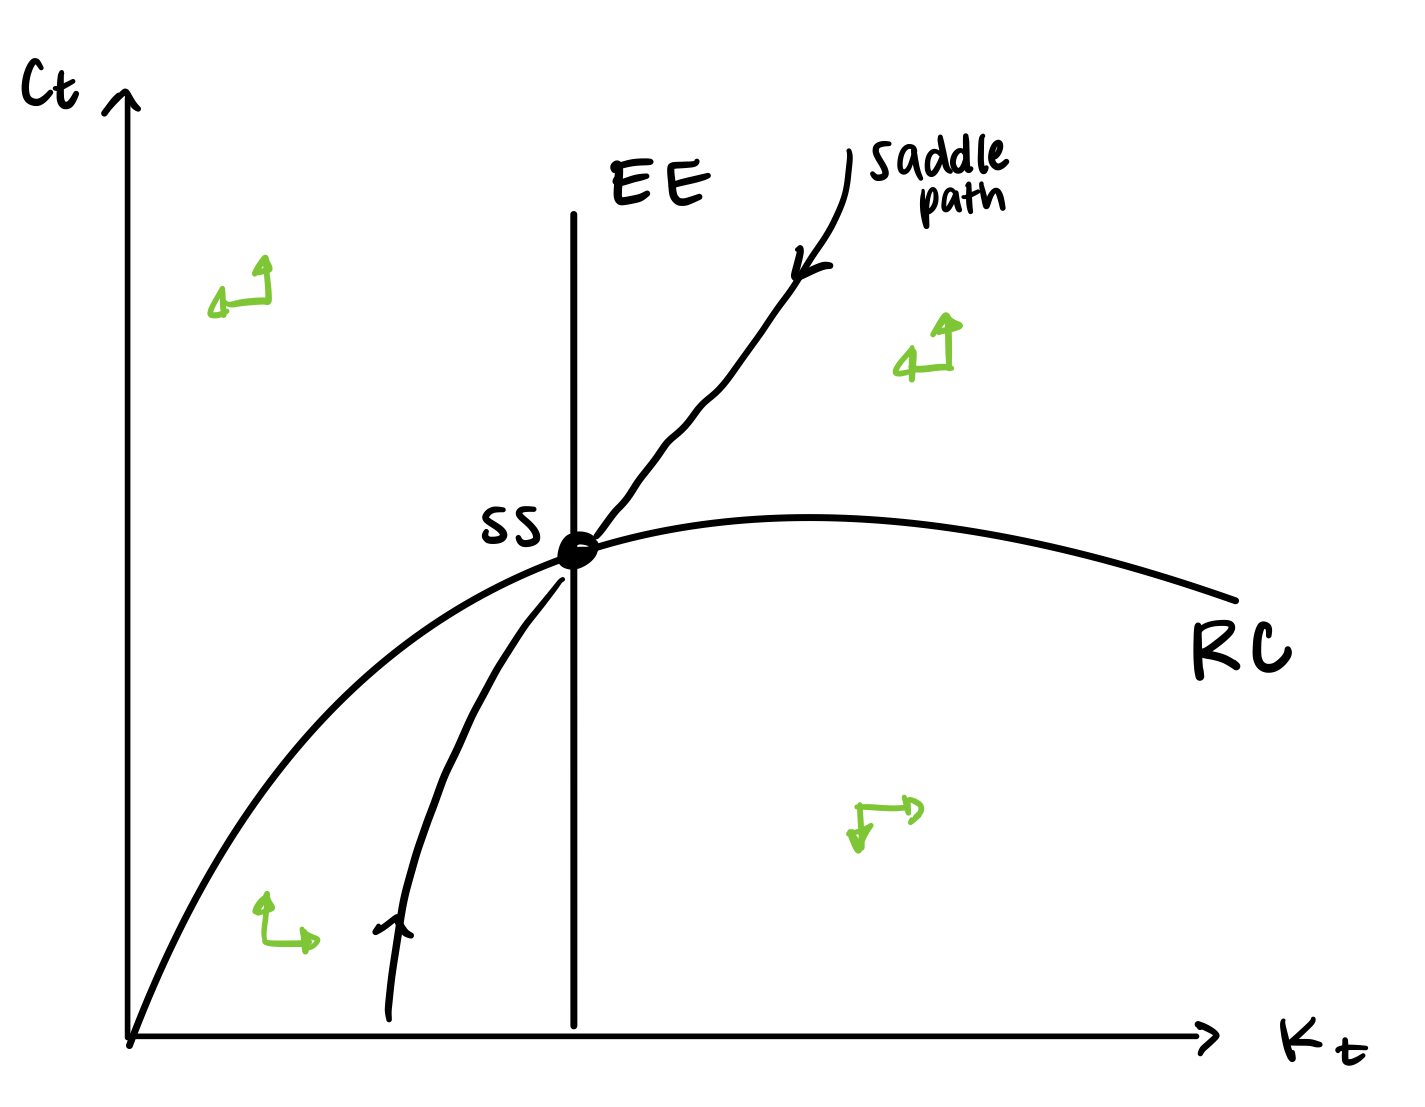
\includegraphics[scale=.3]{q2phase}

\pagebreak
\section{The  scientists  forecast  an  earthquake $T$ periods  from  now  that  will  destroy $D >0$ units of capital.  Assuming that economy starts from a steady state with $D= 0$, draw a phase diagram that shows the optimal transition path.  Make two separate graphs showing the evolution of capital and consumption in time.}
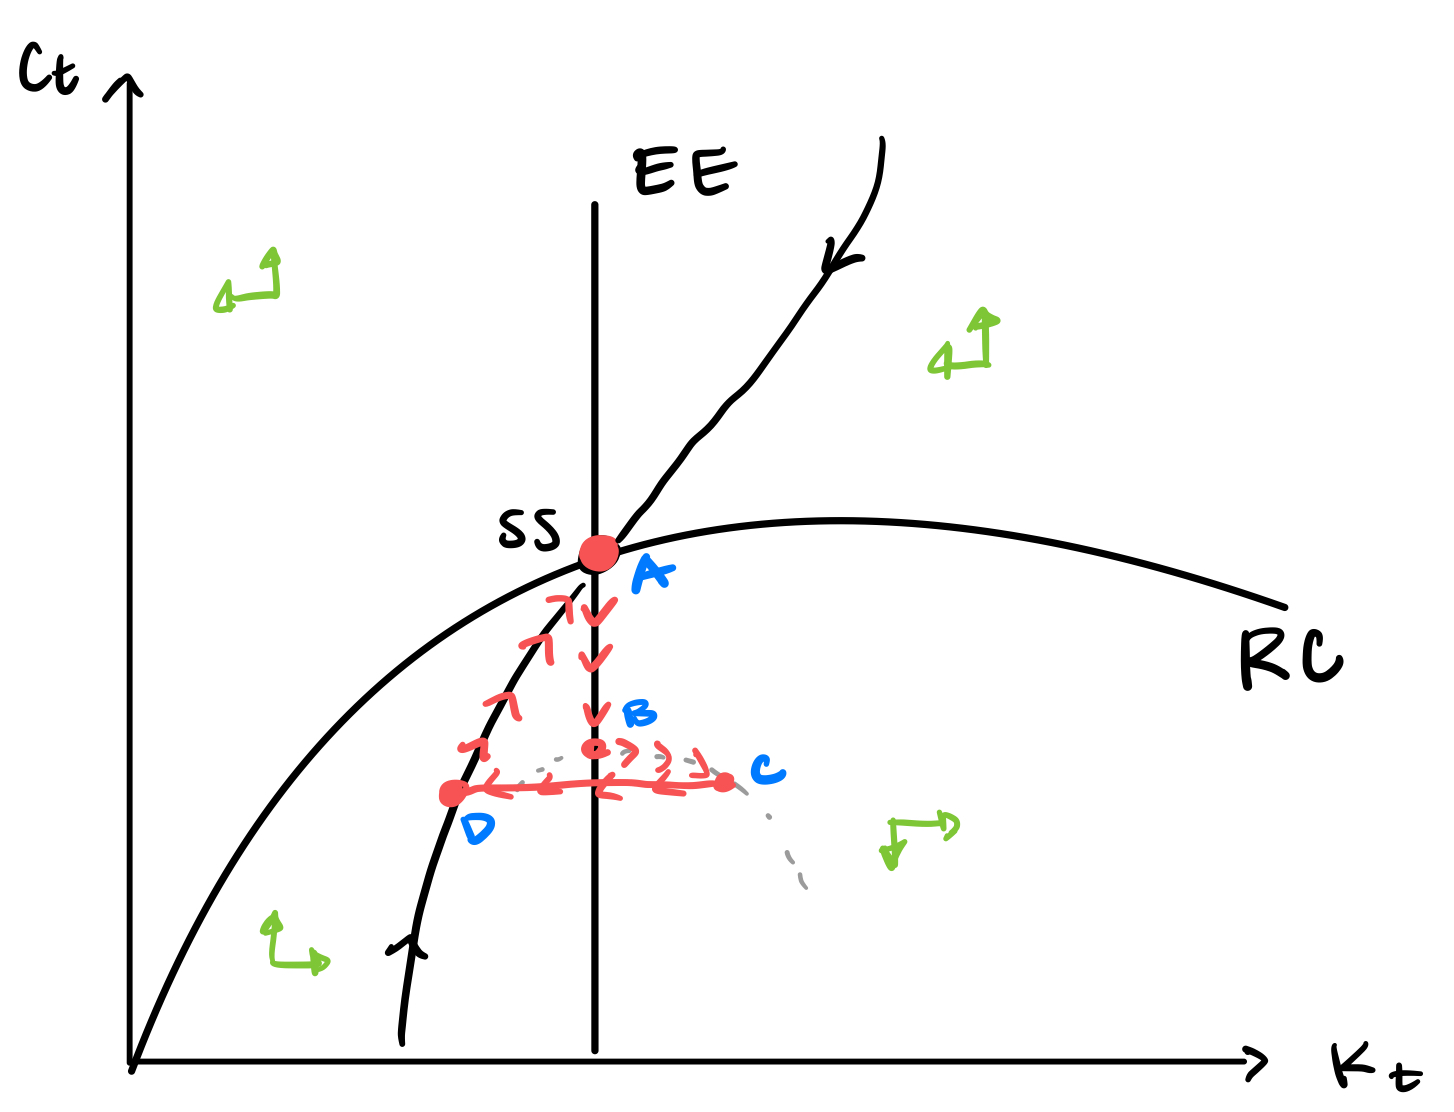
\includegraphics[scale=.2]{q31} \\
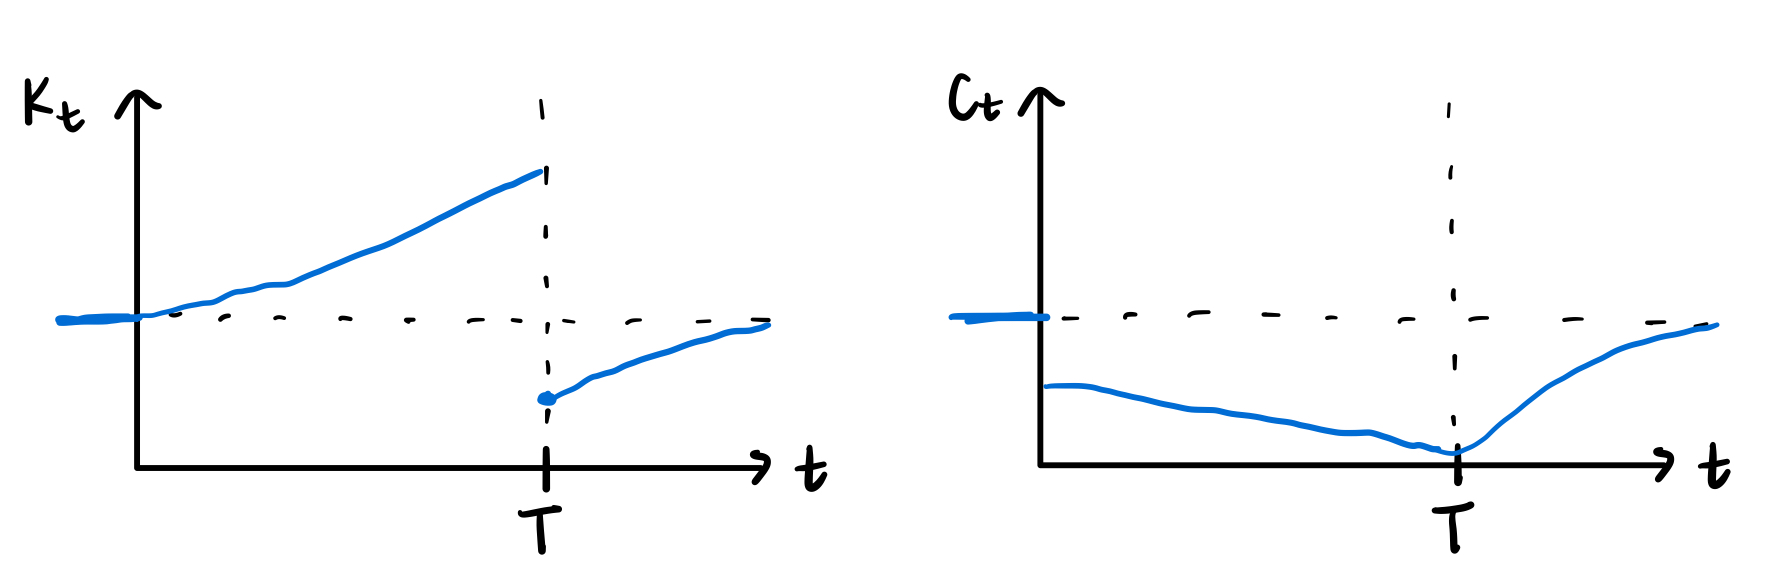
\includegraphics[scale=.2]{q32}

\pagebreak

\section{Assume that $U(C) = \frac{C^{1-\sigma}-1}{1-\sigma} $ and $F(K)= K^\alpha$ and the values of parameters are $\sigma= 1,\;\alpha= 1/3,\;\beta= 0.99^{1/12}$ (monthly model), $\delta = 0.01,\; T= 12,\;D= 1$.  Using a shooting algorithm,  solve  numerically  for  the  optimal  transition  path  and  plot  dynamics  of consumption and capital.}
Updated Euler Equation:
\begin{align*}
% C_t^{-\sigma} & = \beta C_{t+1}^{-\sigma} [\alpha K_{t+1}^{\alpha-1}+1-\delta] \\
C_{t+1} & = \beta^{1/\sigma} C_t  [\alpha K_{t+1}^{\alpha-1}+1-\delta]^{1/\sigma}
\end{align*}
Updated resource constraint:\footnote{\emph{Note: }SS before shock: K = 170.57 and C = 3.84.}
\begin{align*}
K_t^\alpha = C_t + K_{t+1} -(1-\delta)K_t +D_t
\end{align*}


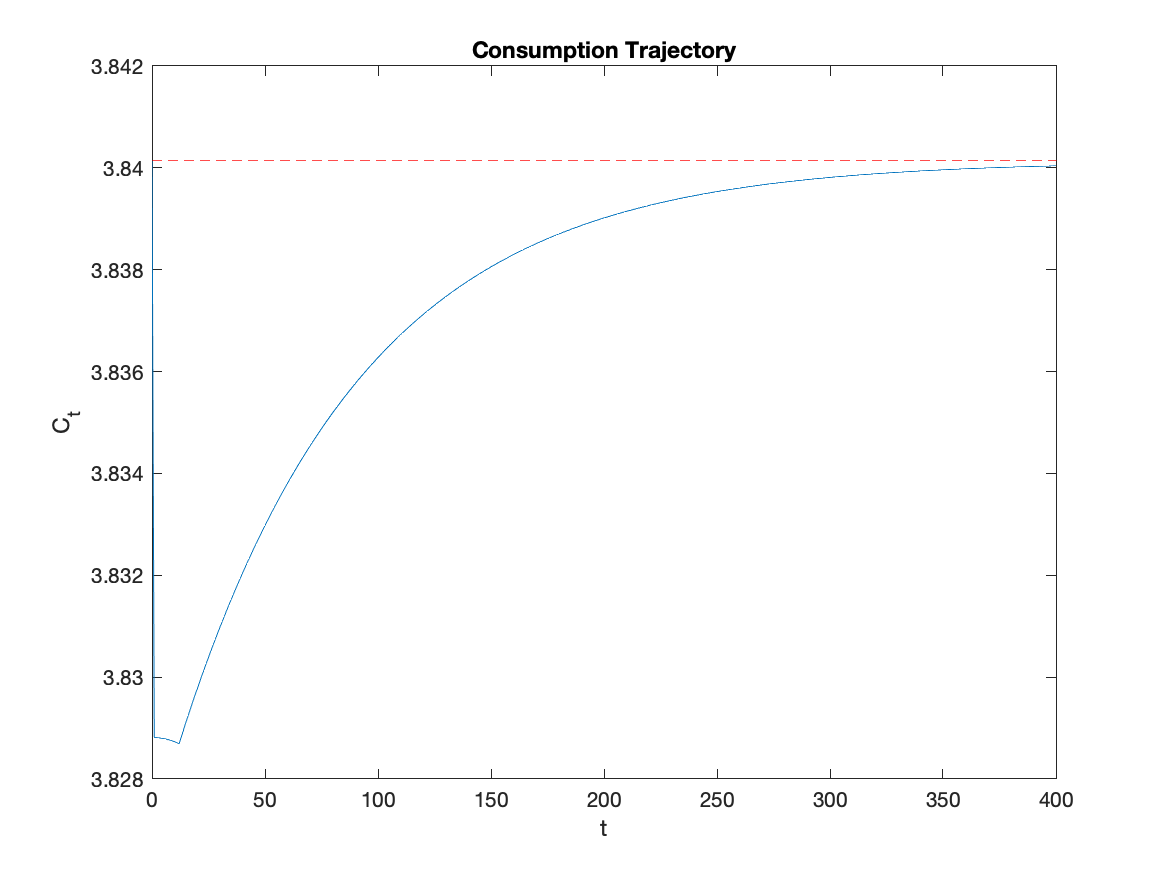
\includegraphics[scale=.7]{consumption}\\
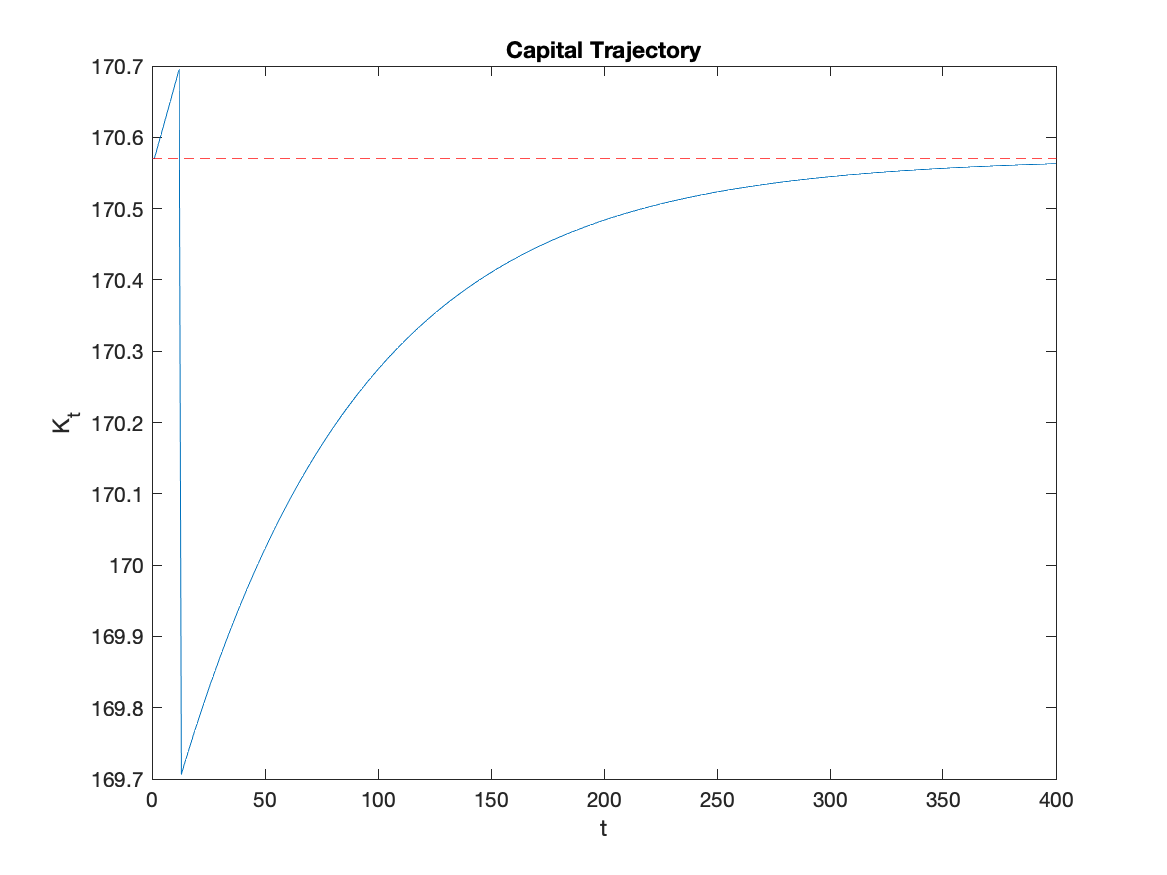
\includegraphics[scale=.7]{capital}




\end{document}
